% MICCAI 2027 draft (LNCS). Numbers: WSI_debate/narval_results; figure: analysis/fig_miccai.py. TODO markers = to fill / verify.
\documentclass[runningheads]{llncs}
\usepackage[T1]{fontenc}
\usepackage{graphicx,booktabs,amsmath,amssymb,xcolor,multirow}
\usepackage[hidelinks]{hyperref}
\newcommand{\todo}[1]{\textcolor{red}{[TODO: #1]}}
\begin{document}
\title{One Advocate per Diagnosis: Cheap, Robust Evidence Selection for Whole-Slide Image Classification}
\titlerunning{One Advocate per Diagnosis}
\author{Anonymous}
\institute{Anonymous}
\maketitle

\begin{abstract}
Foundation-model features give state-of-the-art whole-slide image (WSI) classification, but encoding every tile is expensive. Recent efficient pipelines let a cheap network choose a few tiles and encode only those with the foundation model. This makes the cheap selector a single point of failure: the expensive model never sees what the selector drops. We show that one compromised selector drives an attention-distilled pipeline to below-chance performance on CAMELYON16, CAMELYON17 and TCGA-RCC, and that even a clean single selector rarely shows the foundation model evidence for the competing diagnosis. Following how pathologists work through a differential diagnosis, we instead give each candidate diagnosis its own cheap \emph{advocate}, which presents the tiles that best support it; a foundation-model \emph{judge}, trained on transcripts in which one advocate is adversarial, compares the evidence. Encoding 12--16 tiles per slide, our method stays within 1--7 points of full-slide foundation-model MIL, is on par with an attention-distilled selector on clean CAMELYON16 and TCGA-RCC slides, and keeps .93 balanced accuracy (CAMELYON16), .72 quadratic $\kappa$ (CAMELYON17) and .87 balanced accuracy (TCGA-RCC) when a selector is compromised, where the single-selector pipeline falls to .32, $-$.24 and .02. On renal cell carcinoma subtyping, advocates present runner-up evidence on 87\% of slides (single selector: 30\%) and recover rare chromophobe cases that the single selector misses.
\keywords{Whole-slide images \and Multiple-instance learning \and Efficient inference \and Robustness}
\end{abstract}

%======================================================================
\section{Introduction}
\todo{clinical opening (clinical collaborator): differential diagnosis in practice; RCC subtypes and why heterogeneous tumours / eosinophilic areas make subtyping a comparison between candidates; rare subtypes.}

Pathology foundation models such as UNI~\cite{uni} and CONCH~\cite{conch} make attention-based multiple-instance learning (MIL)~\cite{ilse2018abmil,lu2021data} accurate, but a slide has thousands of tiles and the foundation model must read every one. Efficient pipelines therefore put a cheap network in front of it: ADMIL~\cite{admil2026} distills the attention of a full-slide MIL teacher into an EfficientNet-B0~\cite{tan2019efficientnet} that picks the top-$K$ tiles, and EAGLE~\cite{eagle2026} lets one foundation model select tiles for another. Both report large compute savings at near full-slide accuracy.

These pipelines share one structural property: a \emph{single} selector decides what the expensive model sees. If the selector is wrong---because it is compromised, or simply because it follows the dominant pattern of the slide---the expensive model has no way to recover. This matters most where diagnosis is a comparison: in a differential diagnosis the deciding evidence for the runner-up is often a minority of the tissue.

We make three contributions. \textbf{(1)} We show that an attention-distilled single selector is a single point of failure: one compromised selector drives it below chance on three datasets and every fold, and even when clean it shows the expensive model evidence for the runner-up diagnosis on only 30\% of RCC slides. \textbf{(2)} We propose \emph{one advocate per diagnosis}: cheap per-class selectors present the best evidence for their class, and a foundation-model judge trained with one adversarial advocate compares them. \textbf{(3)} On CAMELYON16~\cite{c16}, CAMELYON17~\cite{camelyon17} (leave-one-hospital-out) and TCGA-RCC~\cite{tcga} we show that this keeps clean accuracy close to full-slide MIL and to the single selector at the same budget, removes the single point of failure, and improves rare-subtype recall over the single selector. We also report what does \emph{not} help (presenter identity, realistic stain shift) and where cheap selection fails for every method (isolated tumour cells).

%======================================================================
\section{Method}
\paragraph{Setting.} A slide is a bag of tiles $\{x_i\}_{i=1}^N$ with label $y\in\{1,\dots,C\}$. Each tile has a cheap view $u_i$ (low magnification, ImageNet EfficientNet-B0, cost $\approx$1\,s per slide) and an expensive view $z_i$ (full resolution, foundation model). A full-slide gated-attention MIL model $F$ on $\{z_i\}$ is the accuracy reference and the source of supervision for the cheap scorer.

\paragraph{Distilled cheap scorer.} A two-layer MLP $g$ on $u_i$ is trained to regress the full model's per-tile class logits (standardised) and to match its attention distribution (KL, as in ADMIL~\cite{admil2026}). Only training slides are used; at test time $g$ never sees the expensive view.

\paragraph{Advocates.} Advocate $c$ presents $K_c$ tiles that best support class $c$ under $g$. For subtyping (RCC) this is the top-$K_c$ tiles by margin $g_c(u_i)-\max_{c'\neq c}g_{c'}(u_i)$. For metastasis detection the classes are ordered, and advocates follow how each stage presents~\cite{camelyon17}: \emph{negative} presents the least tumour-like tiles; \emph{ITC} the most tumour-like tile and its nearest neighbours; \emph{micro} the most tumour-like tiles within 2\,mm of it; \emph{macro} a farthest-point sample of the top 2\% tumour-like tiles (CAMELYON16: two advocates, top and bottom tiles). Only the $CK_c$ presented tiles are read at full resolution and encoded with the foundation model.

\paragraph{Judge and adversarial transcripts.} The judge $J$ is a gated-attention MIL model over the presented tiles, each tagged with a one-hot of its presenting advocate (and, for CAMELYON17, its position relative to that advocate's first tile). It is warm-started on random tiles and then trained for three rounds on (i) honest transcripts and (ii) transcripts in which one advocate for a wrong class is replaced by a white-box attacker that presents the tiles maximising $J$'s current score for that class. Per slide, inference costs one cheap pass over all tiles plus $CK_c$ foundation-model passes.

\paragraph{Single-selector baseline.} Our ADMIL-style reimplementation uses the same cheap features and distilled attention head, selects the top-$K$ tiles with $K=CK_c$, and feeds them to the frozen full-slide model $F$ (ADMIL's design; no code is public).

\paragraph{Threat model.} A compromised selector is replaced by a white-box attacker with the same budget. For the single selector it presents the $K$ tiles with the highest $F$ score for a wrong class; for ours, one wrong-class advocate is replaced (worst case over wrong classes), and on CAMELYON16 the attacker is adaptive (greedy, aware of the honest tiles). In both cases the attacker reads every tile with the foundation model, i.e.\ it is stronger than a cheap attacker.

%======================================================================
\section{Experiments}
\paragraph{Data.} \textbf{CAMELYON16}~\cite{c16}: 399 breast lymph-node slides, official split (270/129), UNI features of 512\,px tiles at 40$\times$; cheap view at level 2 (128\,px). \textbf{CAMELYON17}~\cite{camelyon17}: 500 labelled slides from 5 hospitals, 4 node stages (318 negative, 36 ITC, 59 micro, 87 macro), leave-one-hospital-out; CONCH features of 448\,px tiles at 0.5\,\textmu m/px (mean 1{,}984 tiles per slide). \textbf{TCGA-RCC}~\cite{tcga}: 882 primary-tumour diagnostic slides (492 clear cell, 283 papillary, 107 chromophobe; we exclude normal-tissue and one unreadable slide), 5-fold patient-level stratified CV, CONCH features as above (mean 4{,}349 tiles). Cheap view: ImageNet EfficientNet-B0 at 112--128\,px. $K_c{=}8$ (CAMELYON16) and $4$ (others), so 16, 16 and 12 tiles are encoded per slide.
\paragraph{Protocol.} 3 seeds (CAMELYON16) and 5 folds $\times$ 3 seeds (others). We report balanced accuracy (BA), AUC, accuracy and, for the ordinal CAMELYON17 stages, quadratic-weighted $\kappa$.

\begin{table}[t]\centering
\caption{\textbf{Main results} (mean$\pm$sd). Encoded: tiles per slide sent to the foundation model. Attacked: one selector replaced by a white-box attacker (Sec.~2).}\label{tab:main}
\setlength{\tabcolsep}{3pt}
\resizebox{\linewidth}{!}{\begin{tabular}{@{}lcccccccc@{}}\toprule
 & \multicolumn{2}{c}{CAMELYON16 (BA)} & \multicolumn{3}{c}{CAMELYON17 ($\kappa$ / acc)} & \multicolumn{3}{c}{TCGA-RCC (BA / acc)}\\\cmidrule(lr){2-3}\cmidrule(lr){4-6}\cmidrule(l){7-9}
method & clean & attacked & clean & & attacked & clean & & attacked\\\midrule
full-slide MIL (all tiles) & .969{\tiny$\pm$.008} & -- & .890{\tiny$\pm$.054} & .809 & -- & .933{\tiny$\pm$.016} & .940 & -- \\
single selector (ADMIL-style) & .943{\tiny$\pm$.014} & .315{\tiny$\pm$.059} & .873{\tiny$\pm$.089} & .815 & $-$.241{\tiny$\pm$.237} & .907{\tiny$\pm$.036} & .926 & .022{\tiny$\pm$.014}\\
\textbf{advocates (ours)} & .942{\tiny$\pm$.010} & \textbf{.931}{\tiny$\pm$.013} & .823{\tiny$\pm$.105} & .802 & \textbf{.715}{\tiny$\pm$.152} & .920{\tiny$\pm$.028} & .926 & \textbf{.866}{\tiny$\pm$.029}\\\midrule
encoded tiles / slide & \multicolumn{2}{c}{16 of $\sim$9{,}700} & \multicolumn{3}{c}{16 of 1{,}984} & \multicolumn{3}{c}{12 of 4{,}349}\\\bottomrule
\end{tabular}}\end{table}

\begin{figure}[t]\centering
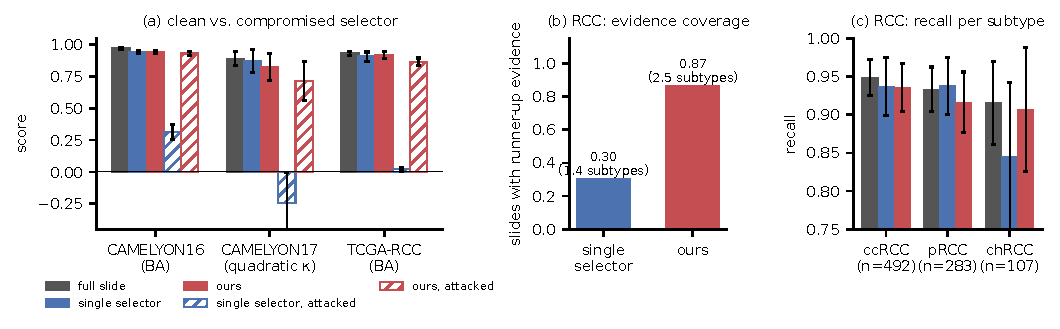
\includegraphics[width=\linewidth]{figs/fig_main.pdf}
\caption{\textbf{(a)} Clean vs.\ compromised selector on three datasets (hatched: attacked). \textbf{(b)} TCGA-RCC: fraction of test slides whose selected tiles include a tile that the full-slide model assigns to the runner-up diagnosis, and mean number of subtypes covered. \textbf{(c)} TCGA-RCC recall per subtype (5 folds $\times$ 3 seeds).}\label{fig:main}
\end{figure}

\subsection{A single selector is a single point of failure}
Table~\ref{tab:main} and Fig.~\ref{fig:main}a: on clean slides the single selector is a strong baseline, within 1--3 points of full-slide MIL while encoding 0.2--0.8\% of tiles. When it is compromised it falls to .32 BA (CAMELYON16), $-$.24 $\kappa$ (CAMELYON17; .03 accuracy on hospital 1) and .02 BA (TCGA-RCC), in every fold and seed. The advocates lose 1--11 points under the same attack: .931, .715 and .866, ahead of the single selector in 15/15 runs on each multi-fold dataset. Robustness is not just redundancy: adding an adaptive attacker to the single selector's tiles in front of the \emph{frozen} full model (no adversarial transcripts) gives .878 on CAMELYON16 vs.\ .931 for ours.

\subsection{Advocates show the judge the competing evidence}
The single selector ranks tiles by one attention score, so it follows the dominant pattern. On TCGA-RCC its tiles contain a tile of the runner-up subtype (as labelled by the full-slide model) on 30\% of test slides and cover 1.4 subtypes on average; advocates cover 2.5 subtypes and show runner-up evidence on 87\% (Fig.~\ref{fig:main}b). This matters for the rare subtype: the single selector recognises 271 of 321 chromophobe test cases (pooled over seeds), advocates 291 and full-slide MIL 294 (Fig.~\ref{fig:main}c; advocates ahead of the single selector in 10/15 runs, behind in 3). Overall BA is .920 vs.\ .907 (ahead in 10/15 runs). \todo{Dr.\ Zhou: tiles of chromophobe cases recovered by advocates and missed by the single selector -- are they diagnostic (perinuclear halos, raisinoid nuclei, plant-like cell borders) and do the single selector's tiles look like eosinophilic clear-cell areas?}

\subsection{Comparison with published MIL on full slides}
On CAMELYON16 with UNI features on every tile, published MIL methods (torchmil~\cite{torchmil} reference implementations, same split, 3 seeds) reach .91--.95 BA (AUC .975--.991): ABMIL~\cite{ilse2018abmil} .946, CLAM-SB~\cite{lu2021data} .914, DSMIL~\cite{li2021dual} .932, TransMIL~\cite{shao2021transmil} .944, DTFD-MIL~\cite{zhang2022dtfd} .926. Advocates reach .942 (AUC .970) while encoding 16 tiles with UNI. \todo{full baseline table in supplement; same on RCC with CONCH?}

\subsection{Ablations and negative results}
\begin{table}[t]\centering
\caption{\textbf{Ablations} (mean over runs). No flags: judge without presenter identity, trained identically. Advocate tiles$\to F$: the advocates' tiles fed to the frozen full-slide model (no judge training). Stain shift: random HED perturbation~\cite{tellez2019stain} of the cheap view of test slides only, none$\to$strength 0.2 (seed 0, 5 folds).}\label{tab:abl}
\setlength{\tabcolsep}{4pt}
\begin{tabular}{@{}lccc@{}}\toprule
 & C16 BA (clean / att.) & C17 $\kappa$ (clean / att.) & RCC BA (clean / att.)\\\midrule
advocates (ours) & .942 / .931 & .823 / .715 & .920 / .866\\
\quad no presenter flags & .937 / .923 & .826 / .719 & .925 / .867\\
\quad advocate tiles $\to F$ & -- & -- & .911 / --\\
single selector & .943 / .315 & .873 / $-$.241 & .907 / .022\\\midrule
stain shift: single selector & -- & .892$\to$.874 & --\\
stain shift: advocates & -- & .815$\to$.790 & --\\\bottomrule
\end{tabular}\end{table}
Table~\ref{tab:abl} lists what does not carry the result. \textbf{Presenter identity} is not needed: a judge without advocate flags, trained the same way, is as accurate and as robust on all three datasets; the gains come from per-class selection plus adversarial judge training. \textbf{Per-class selection alone} is not enough: feeding the advocates' tiles to the frozen full-slide model gives .911 BA on RCC, no better than the single selector. \textbf{Natural stain shift} does not break the single selector: perturbing the cheap view of CAMELYON17 test slides costs both methods $\le$3 points, so the failure mode we study is a compromised or adversarial selector, not routine staining variation.

\paragraph{Limitation: isolated tumour cells.} On CAMELYON17, cheap selection at low magnification misses small metastases for every cheap method: recall for ITC is .03 (full-slide MIL .30) and for micrometastases .25 (advocates) / .36 (single selector) vs.\ .64 (full-slide MIL). The clean $\kappa$ gap to full-slide MIL on CAMELYON17 comes from these stages.

\paragraph{Cost.} \todo{per-slide wall-clock from extraction logs: full-resolution tile reading dominates full-slide inference (e.g.\ $\sim$20--35\,s read vs.\ $\sim$5\,s CONCH per RCC slide); our pipeline reads the low-magnification level ($\sim$2--7\,s), runs B0 ($\sim$1--2\,s) and reads/encodes 12--16 tiles. Fill exact means.}

%======================================================================
\section{Conclusion}
Efficient WSI pipelines that route the foundation model through a single cheap selector are accurate when the selector is right and fail completely when it is not. Giving each candidate diagnosis its own cheap advocate and training the judge against one adversarial advocate keeps the cost of selective inference, keeps clean accuracy close to the single selector and full-slide MIL, removes the single point of failure, and shows the judge the competing evidence, which helps the rare subtype in RCC. Small metastases remain out of reach of low-magnification selection for all methods.

\bibliographystyle{splncs04}
\bibliography{refs}
\end{document}
